\newpage
\section{ Biharmonic Equation}
\label{sec:ch1}


\subsection{Strong form of the Biharmonic Equation}%
\label{sub:strong_form_of_the_biharmonic_equation}


Let $\Omega \subset   \mathbb{R} ^2$ be a bounded polygonal domain and $\partial \Omega $ be its corresponding boundary. Let the fourth order biharmonic equation have the form,

\begin{equation}
\label{eq:bi_problem}
\begin{split}
    \Delta^2  u  + \alpha  u  & = f \quad \text{in } \Omega   \\
    \partial _{n} u & = g_1\left( x \right)  \quad \text{on } \partial \Omega  \\
    \partial _{n} \nabla ^2 u & = g_{2}\left( x \right)  \quad \text{on } \partial \Omega .  \\
\end{split}
.\end{equation}
Here is $\Delta ^2$ the biharmonic operator, also known as the bilaplacian. We will assume for now that $u \in H^{4}\left( \Omega  \right) $, $\alpha $ is a nonnegative constant and $f \in L_{2}\left( \Omega  \right) $. We may consider the functions $g_{1}$ and $g_{2}$ as time independent boundary conditions. Such problems as \eqref{eq:bi_problem} are often associated with the Cahn-Hilliard model
\cite{cahnhilliard1957} for phase seperation. As a matter of fact, the major difference is that \eqref{eq:bi_problem}
has no time dependencie. However, depending on how Cahn-Hilliard model is time discretized numerically can
\eqref{eq:bi_problem} naturally arise. I refer to \cite{brenner2012quadratic} for more informastion on this.

\subsection{Computational Domains}%
\label{sub:computational_domain}

We may want to define the computational domain. Recall that $\Omega \subset   \mathbb{R} ^2$ be a bounded polygonal domain. Let $\mathcal{T} _{h}$ be a triangular mesh of $\Omega$ where every triangle $T \in  \mathcal{T} _{h}$, which is illustrated
in figure \ref{fig:mesh_example}. We define $h$ as
the max diameter of the triangle $T$ such that $h = \max_{T \in \mathcal{T}_{h} }  h_T  $.

\begin{figure}[!h]
    \centering
    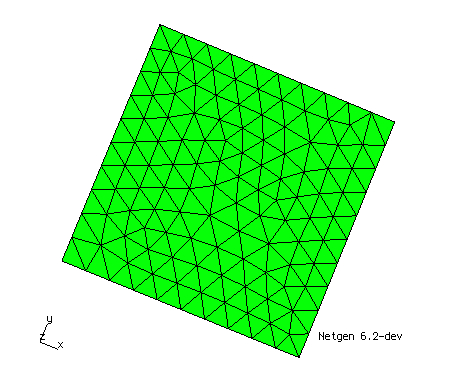
\includegraphics[width=0.45\textwidth]{figures/mesh.jpg}
    \caption{Example of a mesh of $\Omega \subset \mathbb{R} ^{2}$ with triangulation $\mathcal{T} _{h}$.    }
    \label{fig:mesh_example}
\end{figure}

We may also define the set of all edges $\mathcal{F}_{h}$ where every edge is denoted by $E \in \mathcal{F} _{h}$. However, we will distinguish between the
set of external edges $\mathcal{F}^{ext} _{h}$, which is all edges along $\partial \Omega $, and the interior edges $\mathcal{F} ^{int}_{h}$. Let the edges be denotes as $E \in \mathcal{F } _{h}$, then the normal vector $n$ is across the edge from
$T^{+}$ to $T^{-}$, illustraded in figure \ref{fig:normal}.

\begin{figure}[!h]
\centering
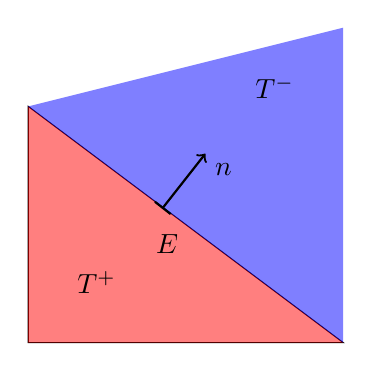
\begin{tikzpicture}[scale=1]
\coordinate (A) at (0,0);
\coordinate (C) at (0,3);
\coordinate (B) at (4,0);
\coordinate (D) at (4,4);
\coordinate (Tm) at (3.5,3.5);
\coordinate (Tp) at (0.5, 0.5);
\coordinate (e) at (1.5, 1.5);
\coordinate (start) at (1.7, 1.7);
\coordinate (end) at (2.25, 2.4);

\draw (A) -- (B) -- (C) -- cycle;
\fill[red, opacity=0.5] (A) -- (B) -- (C);
\fill[blue, opacity=0.5] (B) -- (C) -- (D);
\node[below left] at (Tm) {$T^{-} $ };
\node[above right] at (Tp) {$T^{+}$ };
\node[below right] at (e) {$E$ };

\draw [|->, thick] (start) -- (end);
% \node[above right] at (A) {A };
% \node[below right] at (B) {B};
% \node[above right] at (C) {C };
% \node[below right] at (D) {D};
\node[below right] at (end) {$n$};
\end{tikzpicture}
\caption{Edge $E \in \mathcal{F}_h $ shared by the triangles $T^{+}, T^{-} \in \mathcal{T}_{h} $ and the normal unit vector $n$.  }
    \label{fig:normal}
\end{figure}



\subsection{ Weak Form of Biharmonic Operator in $H^{4} \left( T  \right)$}%
\label{sub:weak_form_biharmonic_identity_for_triangles}


Let $w,v \in  H^{4} \left( T  \right) $ and $\mathcal{T}_{h} $ the simplicial triangulation of $\Omega$. Using the same method as in \cite{gu2012c0, brenner2012quadratic} can we
deduce that for every triangle $T \in  \mathcal{T}_{h} $ it holds that
\begin{align}
        \left( \Delta  ^{2} w, v \right) _{T} &= \left< \partial _{n} \nabla ^2 w, v \right>_{\partial T} - \left( \nabla \left( \nabla ^2 w
 \right), \nabla  v  \right)_{T} \nonumber   \\
\label{eq:weak_form_identity_1}
 &= \left( D^2w, D^2v \right)_{T} + \left< \partial _{n} \nabla ^2 w, v \right>_{\partial T}  - \left<\partial _{n}
 \nabla w, \nabla v \right>_{\partial T} \\
\label{eq:weak_form_identity_2}
 &=  \left( D^2 w, D^2 v \right)_{T} - \left<\partial _{nt} w, \partial _{t} v \right>_{\partial T} - \left<\partial
 _{nn} w, \partial _{n} v \right> _{\partial T} +  \left<\partial _{n} \nabla ^2 w, v \right>_{\partial T}
.\end{align}
Note that we in the second step we used that
\[
    \begin{split}
\left( \nabla \left( \nabla ^2 w \right), \nabla  v  \right)_{T} & = \sum_{i=1}^{2}  \int_{T}^{} \left( \nabla \nabla w_{x_{i}} \right)\cdot  v_{x_{i}} \ dx    \\
 & =  \int_{T}^{} D^2w: D^2v \ dx - \int_{\partial T}^{} \left( \partial _{n} \nabla w \right)
\cdot  \nabla v  \ ds \\
&= \left( D^2 w : D^2v  \right) _{ T} + \left<\partial _{n} \nabla w, \nabla v \right>_{\partial T }  \\
    \end{split}
\]
We denote $D^2$ as the Hessian matrix operator such that
$$( D^2u, D^2v )_{\Omega } = \int_{\Omega }^{} D^{2}u : D^2v  dx,$$
where $D^2u:D^2v$ is the inner product. Also keep in mind that the last result naturally arise when defining $\nabla  = \left( \partial _{n}, \partial _{t} \right) $ such that
\[
\left<\partial _{n} \nabla w, \nabla v \right>_{\partial T} = \left<\partial _{nt} w, \partial _{t} v\right> _{\partial
T} + \left< \partial _{nn} w, \partial _{n} v  \right> _{\partial T} .
\]

Remark that we have two formulations \eqref{eq:weak_form_identity_1} and \eqref{eq:weak_form_identity_2}
\subsection{  Weak Form Biharmonic Equation in $H^{4}\left( \Omega  \right) $}%
\label{sub:continious_weak_form_of_biharmonic_equation}

We might want to introduce the full basic weak formulation of \eqref{eq:bi_problem}. Now, let the solution space be on the form,
\begin{equation*}
V = \left\{ v \in H^2\left( \Omega  \right) : \partial _{n} v = g_{1}  \text{ on }
\partial \Omega  \right\}.
.\end{equation*}

Consider the weak formulation to solve for a $u \in  V$ such that
\begin{equation}
    \label{eq:bi_weak1}
a\left( u,v \right) = F(v).\quad \forall v \in
V.
\end{equation}

By using the identity \eqref{eq:weak_form_identity_1} and utilizing the solution space can we easily do a global summation over the triangulation. Hence, the global weak formulation can be expressed as,
\[
    \begin{split}
\left( \Delta ^2 u, v \right) _{\Omega }  &= \sum_{T \in \mathcal{T} _{h}}^{}  - \left( \nabla  \Delta  u , \nabla v   \right)_{T } + \left<\partial _{n} ( \Delta u ),  v \right>_{\partial T } \\
& = \sum_{T \in \mathcal{T} _{h}}^{} - \left( \nabla  \Delta  u , \nabla v   \right)_{T } + \left<\partial _{n} ( \Delta u ),  v \right>_{\partial T } \\
&= \sum_{T \in \mathcal{T} _{h}}^{}  \left( \Delta u, \Delta v \right)_{T } - \underbrace{\left< \partial _{n} \nabla u,v  \right>_{\partial T }}_{\left< \nabla g_{1},v \right> _{\partial T } }  +  \underbrace{\left<\partial _{n} ( \Delta u ) ,  v
\right>_{\partial T }} _{\left<g_2 ,v \right>_{\partial T } } \\
&=   \left( \Delta u, \Delta v \right)_{\Omega  } - \left< \nabla g_{1},v \right> _{\partial \Omega  }   +  \left<g_2 ,v \right>_{\partial \Omega  }
    \end{split}
\]
such that
\[
    \begin{split}
a\left( u,v \right)_{\Omega } & =    \left( D ^2 u , D ^2 v\right)_{\Omega }  +
\alpha \left( u, v \right)_{\Omega }  , \\
F\left( v \right)_{\Omega } & = \left( f,v \right)_{\Omega } - \left<g_{2},v \right>_{\partial \Omega } + \left<\nabla g_{1}, \nabla v \right>_{\partial \Omega }.
    \end{split}
\]

 In fact, the solution is unique for $\alpha  > 0$. However, for $\alpha  = 0$ must we assume the solvability condtion,
\begin{equation*}
 \int_{\Omega }^{} f dx = \int_{\partial \Omega }^{} g_{2} ds
.\end{equation*}
This condition easily arise when using the substitution $v=1$ in \eqref{eq:bi_weak1}. To handle this, can we extended the solution space \[
V^{*} = \begin{cases}
    V \quad & \alpha  > 0 \\
    \left\{ v \in V: v\left( p_{*} \right)  = 0\right\}, \quad & \alpha  = 0
\end{cases}
\]
where $p_{*}$ is a corner of the polygonal domain $\Omega $.
Thus, the unique solution in $v \in V^{*}$ belongs to $H^{3 }\left( \Omega  \right) $ and we get the follwing
elliptic regularity estimate \cite{gu2012c0},
\begin{equation}
\label{eq:bi_harmonic_ellitpic_regularity}
\left| u \right| _{H^{3 }\left( \Omega  \right) }  \le C_{\Omega } \left( \| f \|_{  L_{2}( \Omega ) }^{  } + ( 1 + \alpha  ^{\frac{1}{2}}
) \cdot \| w  \|_{ H^{4}\left( \Omega  \right)  }^{  }    \right), \quad w\in H^{4}\left( \Omega  \right).
\end{equation}
This regularity estimate may be important for further usecases in terms of error analysis.

